\chapter{Filtrage}

\paragraph*{Idée générale}
Le but de ce chapitre est de décrire les différentes méthodes de filtrage investiguées, dans le but d'améliorer la qualité des données.

\paragraph*{Problème}
Le dataset original est composé de 18 caméras regroupant environ 1 million d'images. Une bonne partie de ces images sont des faux positifs. Il est donc nécessaire de filtrer les images afin de ne garder que les images qui nous intéressent. Une première observation nous fait remarquer que les images uniquement constituées de feuilles n'ont jamais d'animaux. Ensuite, une deuxième lecture nous fait remarquer que les animaux se déplacent plus facilement par temps humide. Et finalement, nous constatons que les animaux sont nombreux certains jours. À partir de ces observations, nous avons élaboré 3 méthodes pour filtrer les images et ainsi augmenter notre probabilité de trouver des animaux pour constituer de nouveaux labels ou constituer un dataset de validation.
Ces méthodes sont décrites dans les sections suivantes.






\section{Analyse des données labellisées}

Comme dit en introduction, notre professeur monsieur Satizabal Mejia Hector Fabio nous a fourni 

un fichier csv contenant les labelisations de 2020 images --> NON --> investiguer !!!!!! (check avec Joris d'où il a pris les données path\_and\_bounding\_box.csv

\subsection{Analyse temporelle}

\subsection{Analyse météorologique}







\section{Détecteur de planches}

Nous avons développé un réseau de neurones convolutif à l'aide de la libraire PyTorch. Ce classificateur binaire, prédit ou non la présence de planche.

\paragraph*{Dataset d'entraînement}

Nous avons extrait 600 images d'une même caméra et labellisé 359 non planches et 241 planches. Ensuite, nous avons développé un dataloader permettant d'intégrer nos labels et de charger des batchs de données directement dans la libraire PyTorch. Celui ci, utilise un pipeline d'entrée qui applique plusieurs transformations à l'image avant de pouvoir l'utiliser comme un tenseur.

\begin{figure}[!htb]
    \centering
    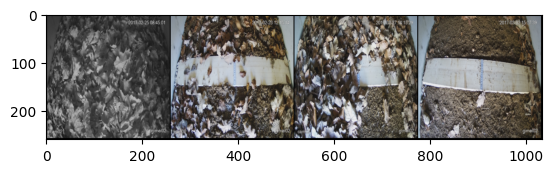
\includegraphics[width=200px]{images/filtre_exemple_data}
    \caption{Exemple de données d'entraînement}
    \label{fig:Entraînement du filtre}
\end{figure}

\paragraph*{Architecture du Détecteur}

Le détecteur est simplement constitué de 3 couches convolutives suivi de 2 couches entièrement connectées. Les channels d'entrée et de sortie des couches convolutives est de : 3 - 32, 32 - 64, 64 - 128. Le nombre de neurones des couches fully connected sont de 128 et 1 pour le neurone de sortie. La fonction de coût utilisé est la BCELoss et l'optimiseur est Adam. Le réseau est entraîné pendant 10 epochs avec un learning rate de 0.001 et un momentum de 0.9 sur 3 epochs.

\begin{figure}[!htb]
    \centering
    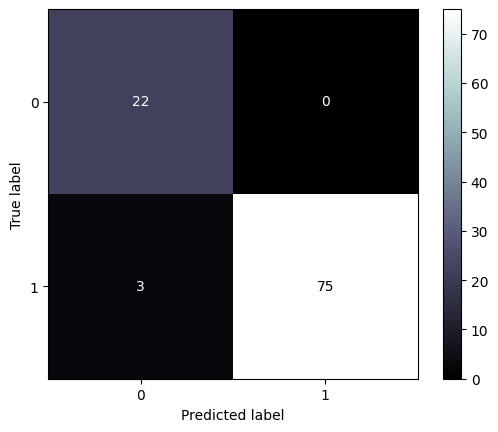
\includegraphics[width=200px]{images/filtre_cmatrix}
    \caption{Matrice de confusion du détecteur de planche}
    \label{fig:Matrice de confusion du filtre}
\end{figure}

\paragraph*{Résultats}

Le détecteur de planche a une précision de 1 et un recall de 0.98 sur la détection de planche. En revanche, la précision sur la détection de non planche est de 0.88 et un recall de 1. Ce qui veut dire que notre filtre est un peu trop efficace et a tendance à se tromper pour détecter les images sans planche. Comme les résultats sont satisfaisant pour dégrossir le travail, nous n'avons pas passé de temps supplémentaire à optimiser le réseau afin qu'il sépare mieux les images dotés d'une planche ou non. Comme, nous traitons une grande quantité de données, l'erreur est acceptable. Lancé sur la quasi intégralité du dataset, le filtre a tourné pendant plus de 10h sur un ordinateur de bureau doté d'un processeur Ryzen9500X. Au final, le filtre a détecté 48910 images de non planches sur les 754543 images analysées.